\newcommand{\danger}{\faIcon{exclamation-triangle}}

\chapter{State of the Art} \label{chap:sota}

%\usepackage{caption}

 In this initial phase of the project, the deliverable pieces are as follows:

 \begin{itemize}
     \item Background, consisting of:
     \begin{itemize}
         \item Frameworks
        \item IDE
        \item Others
    \end{itemize}
     \item Existing Solutions
 \end{itemize}


\section{Background}

Dharma Network's technical foundation is built upon the Algorand blockchain, a \textit{leading blockchain platform} known for its scalability, security and efficiency. The utilization of \textit{Elixir}, \textit{Phoenix} and \textit{Python }technologies enables the development of robust and performant backend services, ensuring seamless interactions between the Dharma Network frontend and the blockchain infrastructure.

As it is an extensive project, Dharma Network compiles an extraordinary variety of languages and frameworks.
For the frontend, it uses \textit{Typescript} and \textit{VueJS}, although this report will focus on the backend and blockchain section. \newline

\subsection{Backend technologies and frameworks}

In the world of software development, the backend plays a crucial role in powering applications and enabling seamless communication between the user interface and the underlying data and systems.\newline

The backend services are mostly written in Elixir, with some functionalities implemented in TEAL, Tealish and Python, with the help of PyTEAL.

\subsubsection{Elixir}\label{elixir}

\textit{Elixir}\footnote{\href{https://elixir-lang.org}{Elixir} is a fault-tolerant, low-latency, dynamic language that is used for building scalable and maintainable applications, such as Discord and Heroku} is a functional programming language based on \href{https://www.erlang.org}{Erlang}\footnote{For a further understanding on Erlang, please check: https://www.erlang.org} \cite{elixir}. \newline

A \textit{functional programming language} consists of developing software with pure functions to create maintainable code. Every function needs to return something and those functions can be used as anything, from variables to arguments. It creates clean and elegant code with immutable data, unlike imperative programming, which doesn't have immutability as a core principle. Functional programming focuses on what needs to be done by defining the relationships and transformations of data. For this matter, errors can quickly be identified and corrected \cite{func}.\newline

Some \textit{key principles of functional programming} are:

\begin{enumerate}
    \item \textit{Pure Functions:} In functional programming, functions are pure, meaning they do not have any side effects and always produce the same output given the same input. Pure functions avoid shared state and mutable data, resulting in more predictable and testable code.
    \item \textit{Immutability:} Data in functional programming is immutable, meaning it cannot be modified once created. Instead of updating values in place, new data structures are created, facilitating a more controlled and predictable system state.
    \item \textit{Higher-Order Functions:} Functional programming encourages the use of higher-order functions, which treat functions as first-class citizens. This allows functions to be passed as arguments, returned as values and composed together, leading to more modular and reusable code.
    \item \textit{Recursion:} Instead of using loops for iteration, functional programming favors recursion. Recursion allows functions to call themselves, enabling elegant and concise solutions to complex problems \cite{func}.
\end{enumerate}

With this being said, some \textit{benefits of functional programming} are:

\begin{itemize}
    \item \textit{Modularity and Reusability:} By promoting the use of pure functions and immutability, functional programming enables developers to create small, composable functions that can be reused in different contexts. This modularity leads to code that is easier to maintain and extend.
    \item \textit{Concurrency and Parallelism:} Functional programming encourages the use of immutable data, which eliminates the need for locks and synchronization. This makes it easier to reason about concurrent and parallel execution, allowing for efficient utilization of modern hardware.
    \item \textit{Error Handling:} With its emphasis on immutability and pure functions, functional programming provides a natural way to handle errors. By separating the pure computation from the error handling logic, developers can write more robust and predictable error handling code \cite{func}.
\end{itemize}

\textbf{Modules in Elixir}\newline

In Elixir, code is organized into modules. A module is a collection of functions, data types and state. It serves as a unit of code organization and encapsulation, enabling developers to group related functionality together. Modules are defined using the \texttt{defmodule} keyword followed by the module name.

Within a module, functions are defined using the \texttt{def} keyword. These functions can be public or private, where public functions are accessible from other modules, and private functions are intended for internal use within the module. Elixir follows the convention of naming files after their corresponding module, allowing for easy navigation.

Modules also support the concept of behaviors, which define a set of functions that a module must implement. Behaviors enable the creation of generic code that can be reused by multiple modules.\newline

\textbf{Mix: Build Tool and Dependency Manager}\newline

\textit{Mix} is a central component of the Elixir ecosystem. It serves as a build tool, task runner and dependency manager for Elixir projects. \textit{Mix} provides a range of tasks, such as compiling code, running tests, managing dependencies and generating documentation. It automates common development tasks and makes it easy to manage the project's lifecycle.

One of the key features of Mix is its dependency management system. With a simple configuration file \texttt{(mix.exs)}, developers can specify the required dependencies for their project. Mix fetches, compiles and manages these dependencies, ensuring that the project's dependencies are correctly resolved and up to date.

Mix also supports the creation of new projects from predefined project templates, allowing developers to quickly bootstrap their applications with a predefined structure and initial configuration.\newline


\subsubsection{Phoenix Framework}

\textit{Phoenix}\footnote{\href{https://www.phoenixframework.org}{Phoenix framework} supports all kinds of resources and languages, such as HTML5, Elixir, database connections, JSON encoding and decoding, etc} is a web development framework written in Elixir and it implements an \textit{MVC} pattern, denominated Model-View-Controller, which means it's divided into 3 layers: \textit{view}, responsible for the interaction with the user; \textit{model}, responsible for the access and manipulation of the data; \textit{controller}, responsible for connecting model and view \cite{phoenix}.\newline

Phoenix works by plugs, its basic element. They come from the Plug library and transform the \texttt{Conn} data structure. This \texttt{Conn} contains every information about the request and response in HTTP connections.\newline

Phoenix's workflow (see figure \ref{fig:phx_work}) can be described as follows:

\begin{enumerate}
    \item Receives a request
    \item Converts request to \texttt{Conn}
    \item \texttt{Conn} passes through several plugs
    \item It renders a response.
\end{enumerate}

\begin{figure}[htbp]
	\centering
	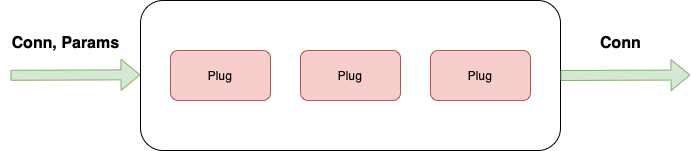
\includegraphics[scale=0.4]{figures/phx_work-3.png}  % largura percentual
	\caption{How Phoenix Works, source: \href{https://blog.logrocket.com/build-rest-api-elixir-phoenix/}{LogRocket}}
	\label{fig:phx_work}
\end{figure}

Let's take a closer look to Phoenix's lifecycle (see figure \ref{fig:phx_lc}):\newline

\begin{figure}[htbp]
	\centering
	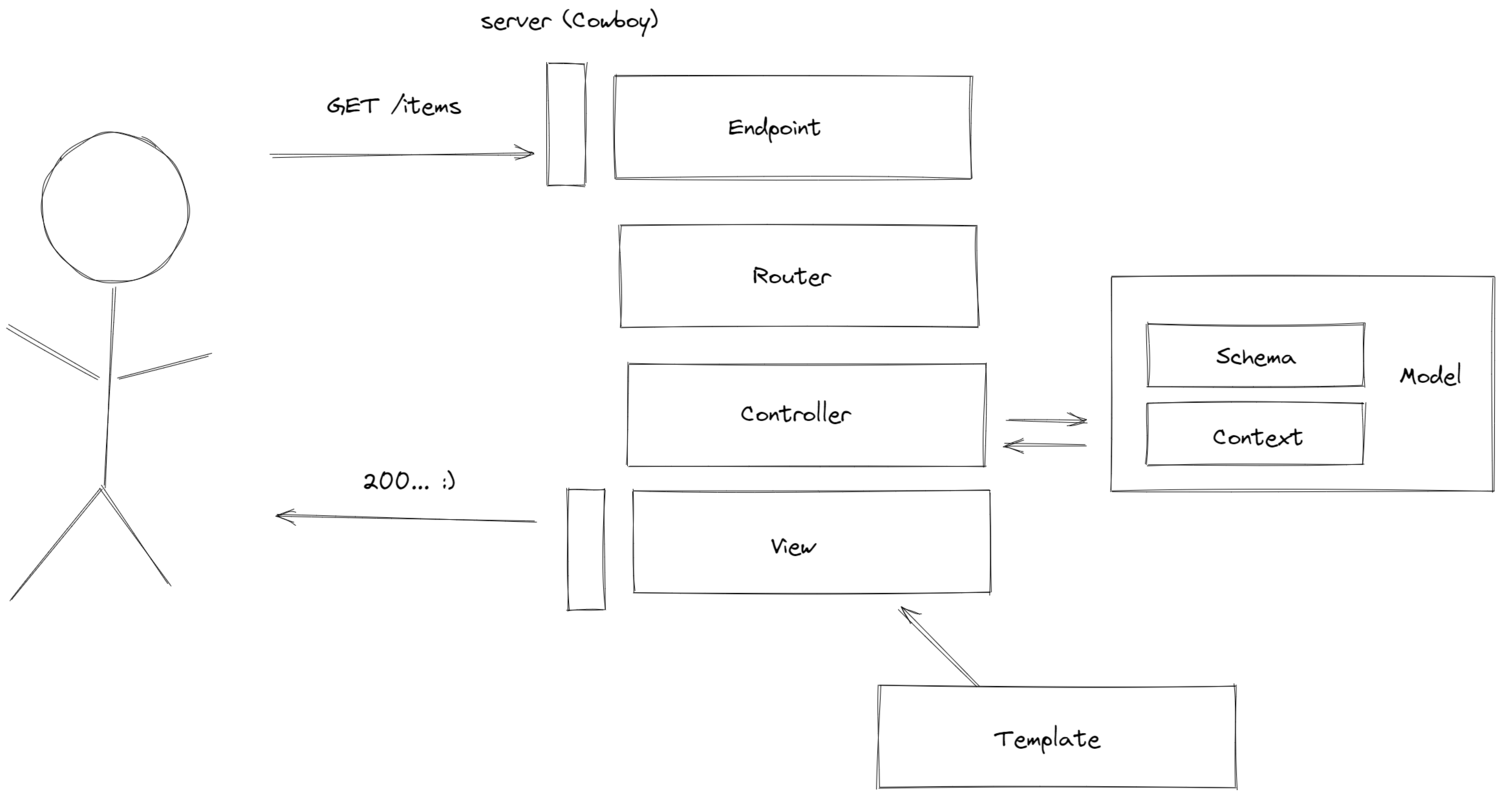
\includegraphics[scale=0.2]{figures/phx_lifecycle.png}  % largura percentual
	\caption{Phoenix's Lifecycle, source: \href{https://serokell.io/blog/introduction-to-phoenix}{Serokell}}
	\label{fig:phx_lc}
\end{figure}

"Phoenix receives a request at the endpoint and the endpoint converts it into a \texttt{Conn} data structure, forwarding it to the router.\newline

The router pipelines the \texttt{Conn} data structure into the controller and the controller interacts with the model to fetch data from the database and render it using templates. Templates can be HTML or JSON files. Here, the endpoint, router and controllers are plugs — everything in Phoenix is a composable function that transforms data into different structure." \cite{phx}\newline


Some advantages of Elixir and Phoenix are:

\begin{itemize}
    \item \textit{Fault-Tolerance and Scalability:} Built on the battle-tested BEAM VM, Elixir and Phoenix provide fault-tolerant capabilities, enabling systems to handle failures gracefully and continue running uninterrupted. Additionally, Elixir's lightweight concurrency model allows for efficient utilization of system resources, making it highly scalable.
    \item \textit{Real-Time and Concurrent Capabilities:} Elixir and Phoenix excel in building real-time applications that require concurrent processing, such as chat systems, collaborative tools and IoT applications. With the built-in support for channels and distributed systems, Phoenix enables developers to create responsive and interactive user experiences.
    \item \textit{Speed:} Elixir and Phoenix are extremely fast, since they compile into BEAM bytecodes and have the speed benefits of Erlang without having the performance issues \cite{adv}.

\end{itemize}


\subsubsection{TEAL}

\href{https://developer.algorand.org/docs/get-details/dapps/avm/teal/}{\textit{TEAL}}, short for "Transaction Execution Approval Language", is the native smart contract language of the Algorand blockchain. It is specifically designed to provide a simple and efficient way to write secure and scalable smart contracts. TEAL is a low-level, stack-based language that operates on Algorand's transactional model. It consists of thirty basic functions.\newline

The main objective of TEAL is to enable developers to express complex logic and conditions that govern the execution of transactions. It allows for the creation of smart contracts that can perform various operations, such as transferring assets, validating conditions and executing custom logic. TEAL contracts are embedded within Algorand transactions, ensuring their atomicity and immutability \cite{teal, teal_2}.\newline

TEAL supports both Stateful and Stateless Smart Contracts (see section \ref{sc}) and those can also be written in Python and compiled by PyTEAL library to TEAL (see section \ref{python} for a further understanding).\newline

To a better understanding of TEAL's workflow, please read section \ref{algo_bc} and see figures \ref{fig:algo} and \ref{fig:algoflow}.

\subsubsection{Tealish}

\href{https://github.com/tinymanorg/tealish}{\textit{Tealish}}, on the other hand, is a higher-level framework introduced by \href{https://tinyman.org}{Tinyman.org}, designed to enhance the development experience of smart contracts on the Algorand blockchain. It provides additional features and abstractions that simplify contract development and improve code readability.\newline

Tealish introduces a more declarative and expressive syntax that abstracts away some of the low-level complexities of TEAL. It allows developers to write smart contracts using a familiar programming style, resembling traditional programming languages. This higher-level abstraction makes contract development more accessible to a broader range of developers.\newline

Furthermore, Tealish focuses on code reusability and composability, allowing developers to create modular contract components that can be easily combined and integrated into larger systems. This modularity enhances code maintainability and fosters the development of scalable and extensible smart contract applications \cite{tealish}.\newline

Some of the \textit{key features and concepts} offered by Tealish include:

\begin{itemize}
    \item \textit{Python-like syntax:} Tealish is designed to resemble the Python programming language, making it familiar and accessible to developers who are already comfortable with Python.
    \item \textit{High-level constructs:} Tealish introduces high-level constructs that abstract away some of the complexities of TEAL, allowing developers to focus on the logic of their smart contracts. These constructs include conditional statements, loops, function definitions and more.
    \item \textit{Static analysis:} Tealish includes a static analyzer that performs checks and provides feedback on potential issues or errors in the code. This helps catch mistakes early in the development process and improves code quality.
    \item \textit{PyTEAL integration:} Tealish seamlessly integrates with PyTEAL, a Python library for compiling TEAL code. This integration allows developers to write their smart contracts using Tealish and then compile them into TEAL using PyTEAL.
\end{itemize}

By providing a higher-level language for writing smart contracts, Tealish aims to simplify the development process and reduce the learning curve associated with TEAL. It can be particularly useful for developers who are more comfortable with Python or prefer a more expressive syntax when working with smart contracts on the Algorand blockchain \cite{tealish}.

\subsubsection{Python}\label{python}

Python is one of the languages that has experienced most growth over the last few years, due to its simplicity and versatility. It also provides a vast library with plentiful resources ready to be implemented, as well as multi platform performance, since the same code can easily be executed on every operative system, whether it's Linux, MacOS or Windows, without the need to be changed.\newline

When it comes to Smart Contracts, in Algorand, they can be written in Python, through the help of \textit{PyTEAL}.\newline

\href{https://github.com/algorand/pyteal}{PyTEAL} allows developers to express complex logic and conditions in a familiar programming language like Python, and then compile it into TEAL.\newline

PyTEAL is a Python library that provides an abstraction layer for writing smart contracts in Algorand. It allows developers to leverage the expressive power of Python to define the logic and conditions of their smart contracts.\newline

Developers can write smart contracts in Python using PyTEAL by defining the desired logic and conditions. They can use Python's control flow statements, variables, functions and libraries to implement the desired behavior of the smart contract.
PyTEAL provides specific constructs and functions to interact with the Algorand blockchain, such as creating transactions, validating conditions and transferring assets.\newline

Once the Smart Contract is ready, it needs to be compiled into TEAL. For that, PyTEAL provides a compilation step that converts the Python code into TEAL bytecode.
The compiled TEAL bytecode can be embedded in Algorand transactions and deployed on the blockchain \cite{pyteal}.\newline

While PyTEAL and Tealish serve similar purposes, there are some \textit{differences} between the two:

\begin{itemize}
    \item \textit{Syntax:} PyTEAL is a \textit{Python library} that allows you to write TEAL code using Python syntax. It provides a way of constructing TEAL programs by using Python functions and constructs. On the other hand, Tealish is a \textit{separate programming language} that resembles Python but is specifically designed for writing Algorand smart contracts. Tealish introduces its own syntax and constructs, which are higher-level than TEAL but still compile down to TEAL code.
    \item \textit{Integration:} PyTEAL integrates directly with the Python ecosystem. It allows you to write TEAL code as Python functions and seamlessly integrate them into your Python-based Algorand applications. PyTEAL provides a convenient way to generate TEAL code using the power and flexibility of Python. On the other hand, Tealish is a standalone language that needs to be separately installed and used alongside PyTEAL. Tealish is used to write the logic of the smart contracts in a more expressive and abstract manner, and then the Tealish code is compiled into TEAL using PyTEAL.
    \item \textit{Abstractions:} Tealish offers higher-level constructs and abstractions that simplify the process of writing smart contracts. It provides a more expressive syntax similar to Python, allowing developers to focus on the logic of their contracts without getting lost in the intricacies of TEAL. PyTEAL, on the other hand, primarily focuses on providing a Python interface for generating TEAL code, but it does not introduce additional abstractions beyond what TEAL itself offers.
\end{itemize}


\subsubsection{Visual Studio Code}

\href{https://code.visualstudio.com}{Visual Studio Code} (VS Code) is a widely popular source code editor developed by Microsoft. It is known for its versatility, extensive plugin ecosystem and cross-platform support. With features like intelligent code completion, debugging support, and Git integration, VS Code enhances developers' productivity and efficiency. Its lightweight nature and customizable interface make it a preferred choice for developers across different programming languages.\newline

All the code was developed on Visual Studio Code.

\subsubsection{PostgreSQL and PG-Admin} \label{post}

\href{https://www.postgresql.org}{\textit{PostgreSQL}} is a powerful open-source relational database management system (RDBMS). It offers robust data integrity, high performance and advanced features, making it a popular choice among developers and enterprises. With support for complex queries, transactions and advanced indexing options, PostgreSQL enables the development of scalable and reliable database-driven applications. Its community-driven development and regular updates ensure its continued growth and relevance in the industry.\newline

The tool used to interact with the database is  \textit{PG-Admin}. PG-Admin is an open-source administration and development platform specifically designed for PostgreSQL. It provides a user-friendly graphical interface that allows users to easily perform various tasks such as creating and managing databases, executing SQL queries, monitoring database performance and much more.\newline

Every database used/created during the internship was PostgreSQL and the main tool used to control it was PG-Admin.\newline


\subsubsection{ITerm 2}

\href{https://iterm2.com}{\textit{ITerm 2}} is an advanced terminal emulator for MacOS. It provides a feature-rich command-line interface, enhancing developers' experience and productivity. \textit{ITerm 2} offers a wide range of functionalities such as split panes, hotkey navigation, session management and extensive customization options. Its support for profiles, triggers and scripting capabilities make it a versatile tool for developers working with command-line interfaces.\newline

\textit{ITerm 2} was used during the project to run and test the code.

\subsubsection{Jira- Atlassian}

\textit{Jira} is a popular project management and issue tracking tool developed by Atlassian. It provides teams with a centralized platform to plan, track and manage software development projects efficiently. With features like task tracking, agile boards, workflow customization and collaboration capabilities, Jira enables teams to streamline their development processes and improve overall project visibility. It integrates seamlessly with other Atlassian tools like Confluence and Bitbucket, creating a comprehensive ecosystem for software development teams.\newline

\textit{Jira} was used during the internship to keep track of the tasks and create new tickets.

\subsection{Blockchain} \label{blockchain}

Blockchain was firstly introduced to the world in 1991, as a way of storing and securing digital data. It consists of a distributed database, otherwise known as ledger, shared among a computer network's nodes. Several parties can access it at once and that particular feature is part of its primary benefit- data can't be altered. In order for a block to be modified, all parties need to be involved, which is a complex procedure, making each block, specifically its data, immutable.\newline

Blockchain works as a peer-to-peer system, making third parties obsolete, such as auditors or other humans that can cause errors and charge fees. Its encryption feature makes it always secure, transactions are done instantly and transparently, since the ledger is automatically updated and the transactions' authenticity is verified and confirmed by its members. \newline

Each new record creates a new block with a unique and identifying hash\footnote{A hash function is a mathematical function that converts a given input value into a shorter, fixed-length value, that represents the original string of characters.}. Blocks are then linked into a chain of records, forming a blockchain \cite{bc}. \newline

For a better understanding of this subject, let's get a closer look of \textit{fundamental components of a blockchain}: \newline

A \textbf{transaction} represents the fundamental units of data exchange within a blockchain network. Each transaction encapsulates essential information, such as sender, recipient and the amount being transferred.

They are cryptographically signed to ensure their authenticity and integrity.\newline

\textbf{Transaction Validation:}\newline

Before a transaction can be included in a block, it undergoes a validation process.
The validation process verifies the transaction's legitimacy, ensuring that the sender has sufficient funds and adheres to predefined rules and protocols.
Validation is performed by network nodes, which collectively maintain the blockchain's consensus mechanism.\newline

\textbf{Transaction Propagation:}\newline

Once validated, the transaction propagates across the network, reaching all participating nodes.
Nodes receive and verify the transaction independently, maintaining a distributed ledger that reflects the transaction's history.\newline


\begin{figure}[htbp]
	\centering
	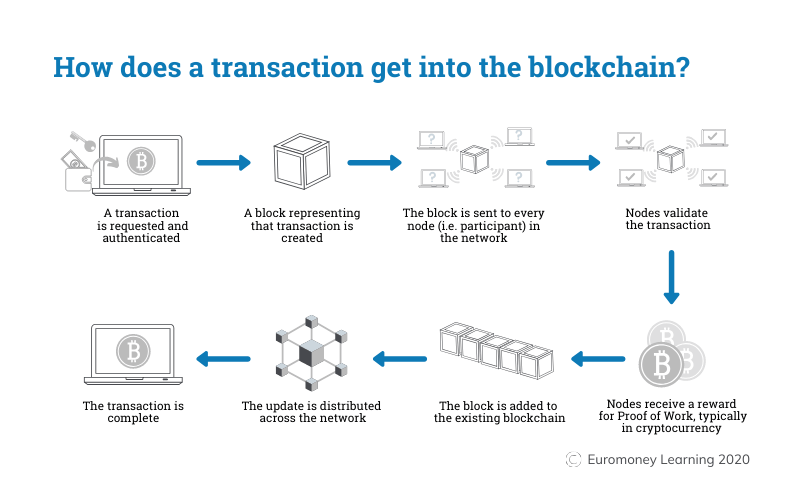
\includegraphics[scale=0.5]{figures/transact.png}  % largura percentual
	\caption{How does a transaction get into the blockchain, source: \href{https://www.euromoney.com/learning/blockchain-explained/how-transactions-get-into-the-blockchain}{EuroMoney}}
	\label{fig:trans}
\end{figure}

A \textbf{block} is a collection of transactions bundled together.
Each block contains a unique hash, a timestamp and a reference to the previous block.
The previous block reference creates a chain-like structure \footnote{Chains are a linked list of blocks. They are immutable and append-only. A blockchain architecture may have one or more chains. Chains can grow to an infinite length or number of blocks. This can be prevented or managed by pruning, but pruning has side effects that reduce the trust in the blockchain network and remove the ability to explore and audit the entire chain. This can reduce the integrity of the chain- \href{https://www.oreilly.com/library/view/hands-on-smart-contract/9781492086116/ch01.html}{O'Reilly}.}, forming the blockchain.\newline


\textbf{Block Formation:}\newline

Miners, specialized participants in the network, compete to add the next block to the chain.
Miners group validated transactions into candidate blocks.\newline
To secure the blockchain, miners must solve a complex mathematical puzzle, known as proof of work, which requires substantial computational power.
The first miner to solve the puzzle broadcasts their solution to the network, earning the right to add their block to the chain.\newline

\textbf{Block Verification and Consensus:}\newline

Upon receiving a new block, network nodes independently verify its validity.
Nodes ensure that the transactions within the block adhere to the predefined rules and protocols.
Consensus mechanisms, such as Proof of Work or Proof of Stake, ensure agreement among nodes regarding the validity of the block.
Block Confirmation and Chain Extension:
Once a block is verified and accepted by the network, it becomes a permanent part of the blockchain.
The block's hash is used as a reference in subsequent blocks, creating an immutable and tamper-resistant record of transactions.
New blocks are added to the chain, extending its length and reinforcing the security of the entire blockchain network.\newline

In the following image (figure \ref{fig:blocks}), it's proposed an example of how the interaction (the evolution of a transaction) between blocks work:\newline

\begin{figure}[htbp]
	\centering
	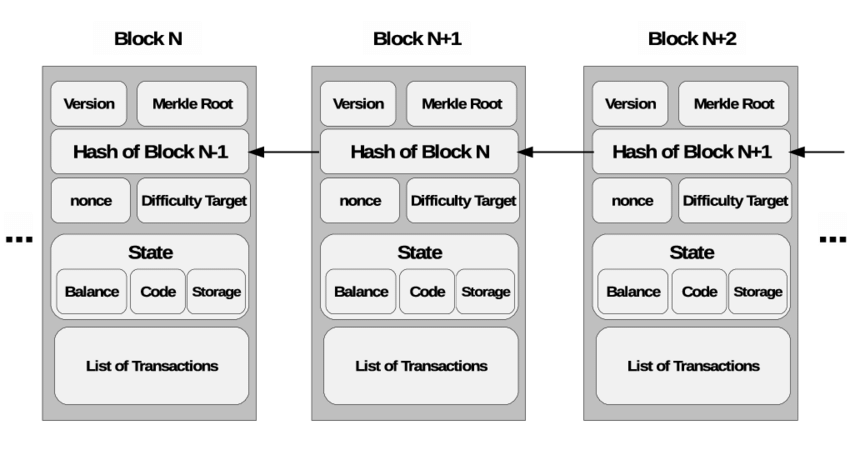
\includegraphics[scale=0.5]{figures/blockchain.png}  % largura percentual
	\caption{Chained blocks creating a blockchain, source: \href{https://www.researchgate.net/figure/Blockchain-design-structure-showing-chained-blocks-with-header-and-body-fields_fig2_321017113}{Research Gate}}
	\label{fig:blocks}
\end{figure}

A \textbf{node} on a blockchain means an electronic device that guards an IP address and it's responsible for running the blockchain's algorithm to verify and authenticate each transaction. They contain a copy of blockchain's primary protocol and its entire transaction history \cite{node}.\newline

Nodes can have 3 various roles when being part of a blockchain \cite{node_type}:

\begin{itemize}
    \item \textbf{Maintaining the blockchain:}
    
Nodes store the data of the blockchain (as mentioned, its primary protocol and transaction history) and help keeping it scalable. 
    
    \item \textbf{Validating a transaction:}

    Some nodes are part of consensus algorithms (see section \ref{cons.mec}), while others just store transaction records. The process involves receiving a transaction order, verifying its authenticity and deciding whether or not to accept it, and recording it on the ledger.
    
    \item \textbf{Accessing information:}

    To access any type of information on the ledger, an interaction with nodes needs to be made. 
\end{itemize}

There are 10 major node types, divided into 4 categories \cite{node_type}:

\begin{enumerate}
    \item \textbf{Full Node:}

    Most ocurrent node. These are responsible for storing the records of the transactions on the ledger. Also defined as the \textbf{servers} of the blockchain. They participate in consensus mechanisms and contribute to the governance of the blockchain. Two types of full nodes are:

    \begin{itemize}
            \item \textbf{Pruned Full Node:}

     These nodes store data on the hard disk by pruning older blocks. They retain a defined amount of recent transaction records, removing the need to store the entire blockchain history. Pruned full nodes strike a balance between storage efficiency and network participation.\newline
    
    \item \textbf{Archival Full Node:}

    As the name suggests, archival full nodes store and maintain the entire blockchain database without any storage limitations. These nodes play a critical role in ensuring the long-term integrity of the blockchain by preserving a comprehensive record of all transactions.
    
Within the category of archival full nodes, there are various specialized nodes:\newline

\begin{itemize}
    \item \textbf{Authority Node:}

    In certain private or partially-centralized blockchains, only a select group of authority nodes have permission to access and manage the blockchain. These nodes exercise control and restrict access to the network.\newline
    
    \item \textbf{Miner Node:}

    Commonly found in Proof of Work-based blockchains like Bitcoin, miner nodes solve complex mathematical problems to validate and add new blocks of transactions to the blockchain. In return for their computational efforts, miners are rewarded with newly minted tokens.\newline
    \item \textbf{Staking Node:}

    These nodes are integral to blockchains utilizing the Proof of Stake consensus model. To participate as a staking node, users must lock a certain amount of native tokens in the network. The blockchain system randomly selects staking nodes to process transactions and record them on the ledger based on predefined rules, such as token holdings or duration of participation.\newline
    \item \textbf{Masternode:}

    Masternodes perform additional functions beyond validating and recording transactions. They serve specific purposes defined by the blockchain network, such as facilitating advanced governance mechanisms or providing specialized services. Dash, an early adopter of masternodes, implemented this concept in its network mechanism.\newline
    
\end{itemize}
    \end{itemize}
    
    \item \textbf{Light Node:}

    Also known as Simplified Payment Verification (SPV) nodes, light nodes store only necessary information such as block headers instead of the entire blockchain. They offer faster transactions and require less storage.

    Designed for efficiency and convenience, light nodes prioritize faster transactions and day-to-day activities. Unlike full nodes, which store the entire blockchain, light nodes store only the necessary information, typically block headers. This streamlined approach reduces storage requirements and allows for quicker synchronization with the blockchain network.\newline
    
    \item \textbf{Lightning Node:}

    These nodes reduce transaction latency by enabling off-chain transactions, minimizing the load on the network and facilitating instantaneous and low-cost transactions.

    When blockchain networks experience high traffic and congestion, lightning nodes come into play. These nodes enable off-chain transactions by establishing direct connections between users, bypassing the need for every transaction to be recorded on the main blockchain. Lightning nodes significantly reduce transaction latency and minimize fees, making microtransactions more viable.\newline
    
    \item \textbf{Super Node:}

    Super nodes perform specialized tasks within a blockchain network, such as maintaining network regulations or implementing upgrades.

    Although less common, super nodes have distinct roles tailored to specific blockchain networks. They may be responsible for maintaining network regulations, implementing protocol upgrades, or supporting specialized functionalities within the blockchain ecosystem.\newline
\end{enumerate}

Understanding the diverse types of blockchain nodes is essential for developers, businesses, and users alike. Developers leverage this knowledge to create efficient decentralized applications, while businesses can optimize their operations and build cost-effective solutions. Users benefit by gaining insights into the underlying infrastructure and making informed decisions based on their specific requirements.\newline

Blockchain nodes are the foundational building blocks of decentralized networks. Their roles collectively contribute to the robustness and reliability of blockchain technology.\newline


A \textbf{fork} occurs when a community proposes changes to the blockchain's protocol or underlying rules, either for efficiency or concerning matters. These changes result in the separation of the blockchain, giving rise to a new blockchain that shares the entire transaction history but embarks on a different path. This way, forks enable DeFi to enhance security, introduce new functionalities, address security risks or create an entire new coin and ecosystem \cite{fork}.


\begin{figure}[htbp]
	\centering
	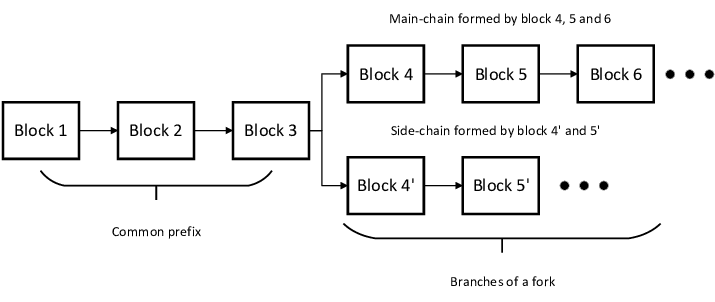
\includegraphics[scale=0.4]{figures/fork.png}  % largura percentual
	\caption{Fork structure, source: \href{https://www.researchgate.net/figure/Fork-structure-in-a-blockchain_fig2_342017074}{Research Gate}}
	\label{fig:fork}
\end{figure}

Forks can be if two main types: soft forks and hard forks \cite{fork}.

\begin{itemize}
    \item \textbf{Soft Forks:}

    Soft forks are analogous to software updates for the blockchain.
When universally adopted by users, soft forks establish new rules for a cryptocurrency.
These are typically employed to introduce new programming functions or features.
As soft forks maintain a single blockchain, the changes are backward compatible with pre-fork blocks. As an example, there's SegWit's upgrade, Bitcoin's Segregated Witness protocol.\newline
    \item \textbf{Hard Forks:}

    A hard fork occurs when the code undergoes significant changes, rendering the new version incompatible with older blocks.
In this scenario, the blockchain splits into two: the original blockchain and a new version adhering to new rules.
Hard forks give rise to entirely new cryptocurrencies, spawning well-known coins such as Bitcoin Cash and Bitcoin Gold, derived from the original Bitcoin blockchain.

\end{itemize}

\begin{figure}[htbp]
	\centering
	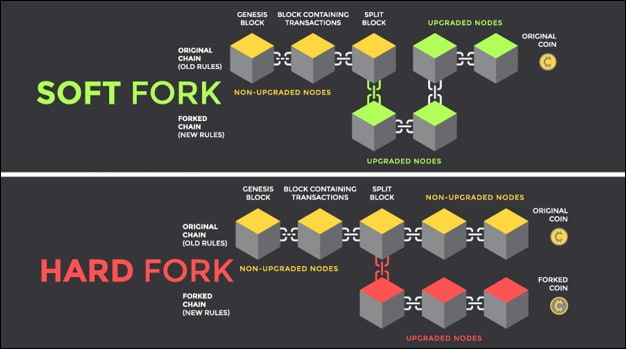
\includegraphics[scale=0.5]{figures/fork_type.jpeg}  % largura percentual
	\caption{Fork types, source: \href{https://shardeum.org/blog/what-is-a-blockchain-fork/}{Shardeum}}
	\label{fig:fork_type}
\end{figure}



\subsubsection{Consensus Mechanism} \label{cons.mec}

To ensure maximum security in each node, there are some mechanisms to approve the addition of a new node to the chain. They are also used to keep the ledger updated in every node. \par
Since blockchain doesn't require third parties, no authority can declare that a certain version of the data is correct and verified, which brings up the question: \textit{how is that veracity proved?} \newline
That's where consensus mechanisms come in. Some of the most popular are \textit{Proof-of-Work (PoW}, \textit{Proof-of-Stake (PoS)} and \textit{Practical Byzantine Fault Tolerant Mechanism}:\newline

\begin{itemize}
    \item \textbf{Proof-of-Work (PoW)}:
    
    PoW is the consensus mechanism used by Bitcoin and many other cryptocurrencies. In PoW, nodes in the network compete to solve complex mathematical puzzles, requiring significant computational power. The first node to solve the puzzle earns the right to add the next block to the blockchain, which means newly minted cryptocurrency.\newline
    This process is resource-intensive and time-consuming, making it difficult for an attacker to tamper with the blockchain. The proof of solving the puzzle is then shared with the network, allowing other nodes to verify and reach consensus on the validity of the new block. The nodes responsible for the problem solving are called miners and its process is called mining. Miners can be rewarded with a certain amount of the cryptocurrency if they contribute to the solution \cite{hack}.

    \item \textbf{Proof-of-Stake (PoS)}: 
    
    PoS is an alternative consensus mechanism that aims to address the resource consumption of PoW. In PoS, the creator of the next block is chosen in a deterministic way, based on their stake or ownership of the cryptocurrency. Instead of solving puzzles, validators, also known as stakeholders, are selected to validate transactions and create new blocks based on their existing stake. Validators are incentivized to act honestly, as their stake can be penalized if they behave maliciously. PoS is considered to be more energy-efficient compared to PoW and allows for faster block generation times \cite{hack}.

    \item \textbf{Practical Byzantine Fault Tolerant (PBFT) Mechanism}: 
    
    PBFT is a consensus mechanism designed for distributed systems, including blockchain networks. It focuses on reaching consensus among a set of nodes even if some of them are faulty or malicious (Byzantine faults). PBFT ensures that the majority of nodes agree on the order of transactions, and once a block is approved by the network, it is considered final. This mechanism is often used in permissioned blockchain networks where the participants are known and trusted \cite{hack}.

\end{itemize}

\subsubsection{Smart Contracts}\label{sc}

Smart contracts are an important and complex part of a blockchain.

These are defined as computer programs stored on a blockchain that automatically execute (when predetermined needs are met) and enforce contractual agreements without the need for intermediaries.

Its structure follow a simple \textit{"if/when...then" logic}, where participants agree upon specific conditions and corresponding actions.
Once the conditions are met and verified by a network of computers, the smart contract automatically executes the specified actions. Let's see an example:\newline

"\textit{(...) \textbf{IF} you send object A, \textbf{THEN} the sum (of money, in cryptocurrency) will be transferred to you.
\textbf{IF} you transfer a certain amount of digital assets (cryptocurrency, for example, ether, bitcoin), \textbf{THEN} the A object will be transferred to you.
\textbf{IF} I finish the work, \textbf{THEN} the digital assets mentioned in the contract will be transferred to me (...)}" \cite{sc}.\newline

Some of its key benefits and features are:

\begin{itemize}
    \item \textit{Autonomy:} Smart contracts operate autonomously, eliminating the need for manual or third parties intervention.
    \item \textit{Self-Enforcement:} They automatically execute contract terms and enforce obligations.
    \item \textit{Immutable:} Contract terms and conditions cannot be altered once deployed on the blockchain.
    \item \textit{Trustless:} Smart contracts rely on cryptographic protocols and decentralized consensus, reducing the need to trust intermediaries.
    \item \textit{Distributed:} They are replicated and distributed across all nodes connected to the network, ensuring all participants have a copy of its conditions.
    \item \textit{Deterministic:} Smart contracts operate based on predefined functions that are executed only when specific conditions are met, so its outcome will remain consistent, regardless of who executes the contract, ensuring predictable and reliable results.
    \item \textit{Customizable:} They offer flexibility for customization and modification before being launched. Users can tailor the contract to meet their specific requirements, adding versatility and adaptability to the agreement.
    \item \textit{Transparent:} Smart contracts are stored on a public blockchain, making the code visible to everyone, regardless of their participation in the contract. This transparency promotes accountability and trust among the parties involved.
    \item \textit{Self-Verifying:} They possess the capability to verify themselves automatically. The predefined conditions and rules are built into the contract, ensuring that they are met at every stage without requiring external verification.\cite{sc}
    
\end{itemize}


\begin{figure}[htbp]
	\centering
	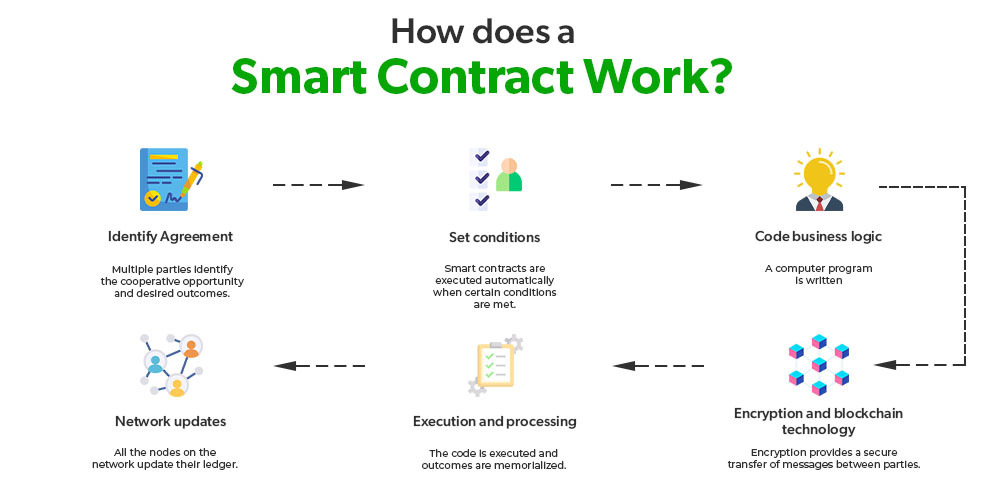
\includegraphics[scale=0.4]{figures/smart.png}  % largura percentual
	\caption{Workflow of a Smart Contract, source: \href{https://www.geeksforgeeks.org/smart-contracts-in-blockchain/}{GeeksforGeeks}}
	\label{fig:smartcont}
\end{figure}

Smart Contracts can be applied in many industries, such as healthcare or real estate, but they will be of tremendous importance when it comes to \textit{management} and \textit{voting} on Dharma Network (more detailed at chapter \ref{chap:chap4}).\newline

Smart Contracts in Algorand (layer-1 smart contracts, or ASC1- see figure \ref{fig:algoprimer}) can be of two types: smart contracts and smart signatures.\newline

\textit{Smart Contracts}, also called \textit{Stateful Smart Contracts}, function as state-holding contracts and store on-chain values globally or for individual accounts. They are initiated by stateful smart contract transactions and process the logic within the contract.\newline 
Stateful smart contracts can be linked with payment transactions using Algorand's Atomic transfer capability (see figure \ref{fig:algoprimer}), which allows multiple transactions to be submitted simultaneously. By leveraging this feature, stateful smart contracts can effectively approve or reject a spending transaction based on the logic they contain. The ABI (\textit{Application Binary Interface}) provides a standard method for exposing APIs and encoding/decoding data types for application call transactions \cite{scalgo, scalgo2}.\newline

\begin{figure}[htbp]
	\centering
	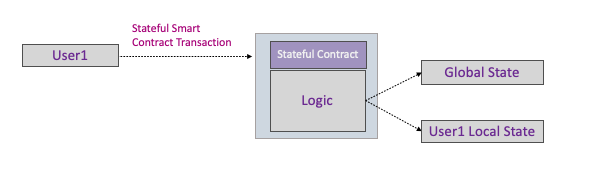
\includegraphics[scale=0.5]{figures/stateful.png}  % largura percentual
	\caption{Workflow of a Stateful Smart Contract, source: \href{https://developer.algorand.org/articles/linking-algorand-stateful-and-stateless-smart-contracts/}{Algorand Developer Portal}}
	\label{fig:stateful}
\end{figure}

On the other hand, \textit{Smart Signatures}, also known as \textit{Stateless Smart Contracts}, are primarily used to approve spending transactions with logic. The logic is submitted with a transaction and evaluated by the AVM. If the logic fails, the associated transaction is not executed. They can be signed by a user's signature, a multi-signature or with the logic of a stateless smart contract itself. \newline
Smart signatures can function as accounts similar to other accounts on the blockchain, allowing funds to leave only if the transaction successfully executes the logic within the smart signature. They can also be used for account delegation, where an account signs the smart signature, which can be used later to sign a transaction from the original signer's account\cite{scalgo, scalgo2}.

\begin{figure}[htbp]
	\centering
	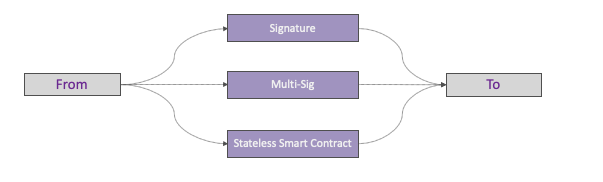
\includegraphics[scale=0.5]{figures/stateless.png}  % largura percentual
	\caption{Workflow of a Stateless Smart Contract, source: \href{https://developer.algorand.org/articles/linking-algorand-stateful-and-stateless-smart-contracts/}{Algorand Developer Portal}}
	\label{fig:stateless}
\end{figure}

Both smart contracts and smart signatures are evaluated by the AVM, with access to limited global variables, temporary scratch space and transaction properties. They play different roles in the Algorand ecosystem, with smart contracts providing decentralized application logic and state management, while smart signatures focus on transaction signing and delegation \cite{scalgo, scalgo2}.

\subsubsection{Types of Blockchain}\label{typesofb}

Blockchains can be split into two main groups: permissionless and permissioned. Each one is used depending on the operation to perform \cite{perm_bc}.

\begin{enumerate}
    \item \textbf{Permissioned Blockchain} is ideal for applications requiring role definition and limited access. Users are added or removed based on digital verification or certificates, offering an additional layer of security and privacy compared to public blockchains \cite{bc_types, perm_bc}.

These are implemented by major companies worldwide due to its security features and they're commonly used in supply chain management, contract creation, identity verification and payment verification.

Some of its features are:

\begin{itemize}
    \item \textit{Transparency:} Clear tracking of changes and user actions.
    \item \textit{Data Security:} Complete control over data access and permission management.
    \item \textit{Lack of Anonymity:} Every change is tracked to individual users, promoting accountability.
    \item \textit{Restricted Authority:} Private groups can authorize decisions without centralized control \cite{perm_bc}.
\end{itemize}

    \item \textbf{Permissionless Blockchain}, also known as public blockchain, is a blockchain open to participation without restrictions. It's a decentralized platform with no central authority or administrator, so the transparency of transactions is available to all participants.
It offers open-source development and limited anonymity \cite{bc_types, perm_bc}.


These are commonly used in financial platforms, digital trading, donations and crowdfunding.\newline

Some of its features are:

\begin{itemize}
    \item \textit{Transparent Transactions:} Complete visibility of transactions to all users.
    \item \textit{Open Development:} Accessibility for users to modify and improve the platform.
    \item \textit{Anonymity:} Participants have certain exceptions to privacy while making changes.
    \item \textit{Lack of Central Authority:} No centralized control or authorization required.
    \item \textit{Token Incentives:} Use of tokens and digital assets to encourage participation \cite{perm_bc}.
\end{itemize}

For a further understanding of the difference between them, see table \ref{tab:blockchain-comparison} to see their comparison and table \ref{proscons} to check their pros and cons.\newline
\end{enumerate}


Inside the world of permissioned and permissionless blockchains, there's 4 types: \textit{public blockchain}, \textit{private blockchain}, \textit{hybrid blockchain} and \textit{consortium blockchain} (see figure \ref{fig:type})\cite{bc_types}.

\begin{figure}[htbp]
	\centering
	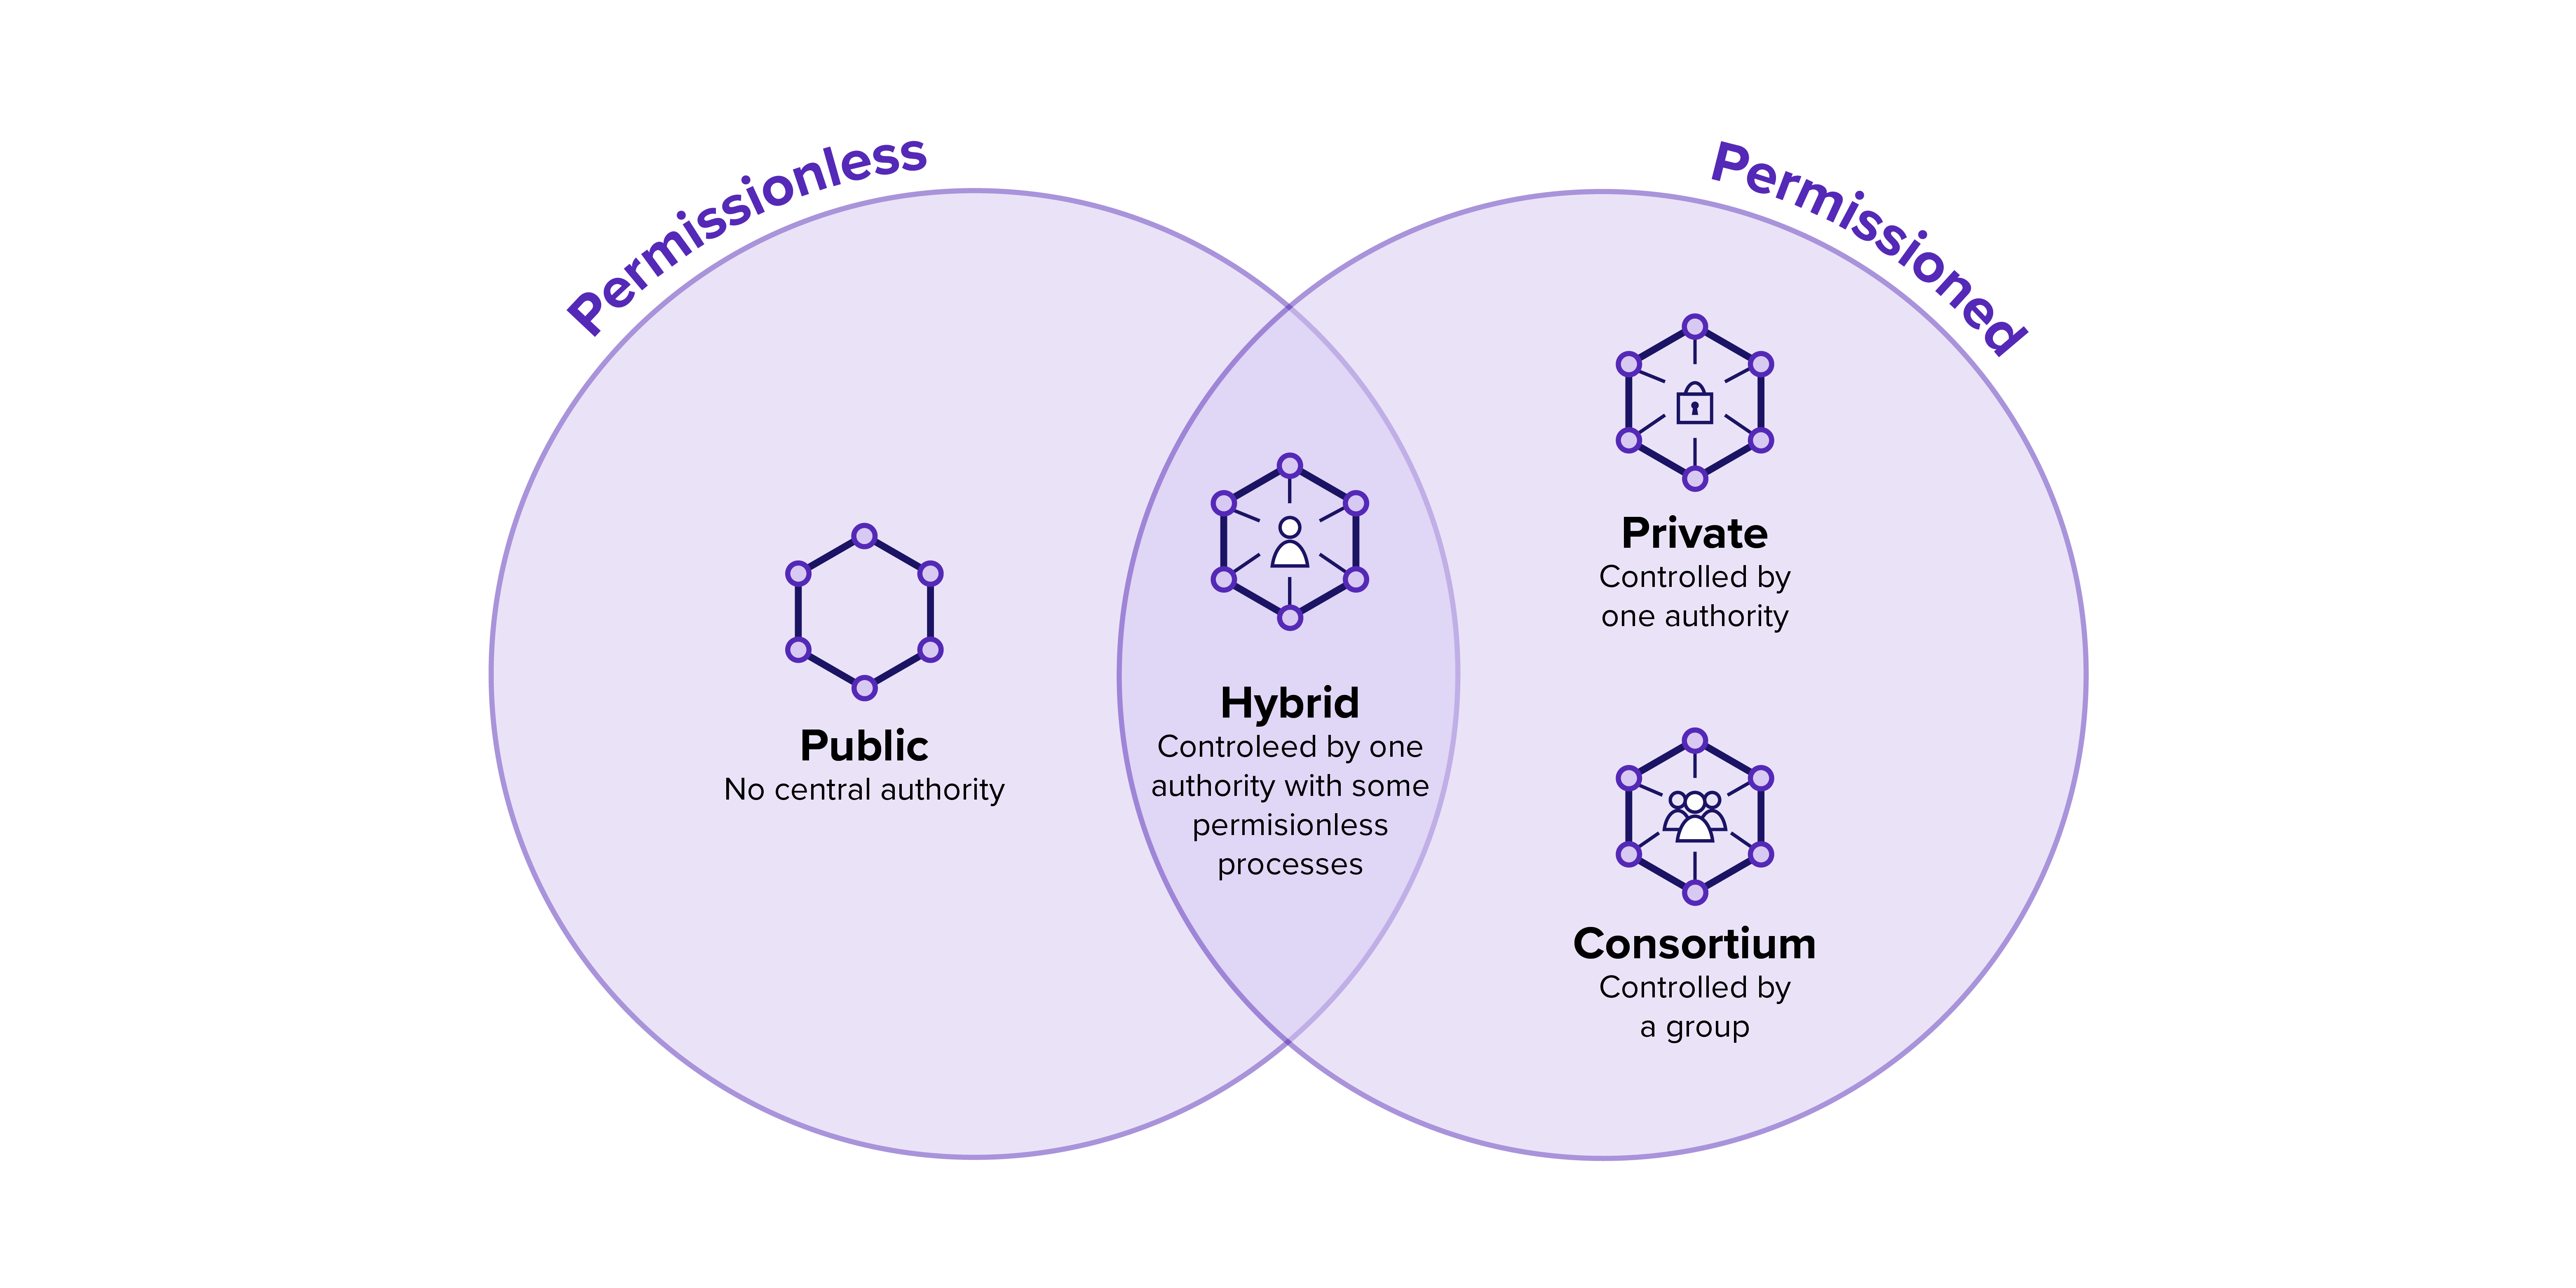
\includegraphics[scale=0.2]{figures/perm.png}  % largura percentual
	\caption{Venn Diagram of Blockchain Types, source: \href{https://www.parcl.co/blog/the-4-types-of-blockchain-and-why-you-should-know-the-difference}{Parcl}}
	\label{fig:type}
\end{figure}

\begin{enumerate}
    \item \textbf{Public Blockchain:}

    Public blockchain operates on a permissionless distributed ledger, allowing anyone to join and participate in transactions. The open nature of public blockchains promotes transparency and trust within the user community. Bitcoin, as one of the earliest public blockchains, enabled decentralized transactions accessible to anyone with an internet connection. However, public blockchains face challenges in scalability and privacy, making them more suitable for applications such as voting and fundraising.
    
    \item \textbf{Private (or Managed) Blockchain:}

    Private blockchains operate in closed networks and are managed by organizations. These blockchains provide a higher degree of control and privacy compared to public blockchains. In a private blockchain, access and permissions are restricted, allowing for faster transactions and scalability. Organizations can employ private blockchains to streamline supply chain management, track asset ownership, or facilitate internal voting processes. However, the centralized nature of private blockchains contradicts the decentralized principles of blockchain technology and security may be compromised due to the limited number of nodes.
    
    \item \textbf{Consortium Blockchain:}

    Consortium blockchains, also known as federated blockchains, combine elements of both public and private blockchains. These blockchains are controlled by multiple organizations, striking a balance between transparency and privacy. Consortium blockchains offer scalability, security, and efficient governance structures. Use cases for consortium blockchains include banking and payment systems, research collaborations and supply chain management. However, the integrity of the member organizations can impact the network's effectiveness, and legal and regulatory factors may influence its operations.
    
    \item \textbf{Hybrid Blockchain:}

    A hybrid blockchain combines features of both private and public blockchains, catering to organizations that require the benefits of both worlds. It allows for private and secure transactions while still being part of a public network. Hybrid blockchains offer flexibility in adjusting rules and providing privacy as needed. Real estate, retail, and highly regulated industries can leverage hybrid blockchains to improve process efficiency and comply with strict regulations. However, the lack of full transparency and the complexity of transitioning to hybrid blockchains are notable considerations.
\end{enumerate}

Understanding the characteristics of each type enables organizations to make informed decisions when adopting blockchain technology, aligning with their goals and industry requirements.

\subsubsection{Algorand Blockchain}\label{algo_bc}

Dharma Network is built on top of Algorand blockchain, as previously mentioned. 

Figure \ref{fig:algoprimer} mentions four essential components that were and will continuously be mentioned in the course of this paper, regarding Algorand blockchain:

\begin{figure}[htbp]
	\centering
	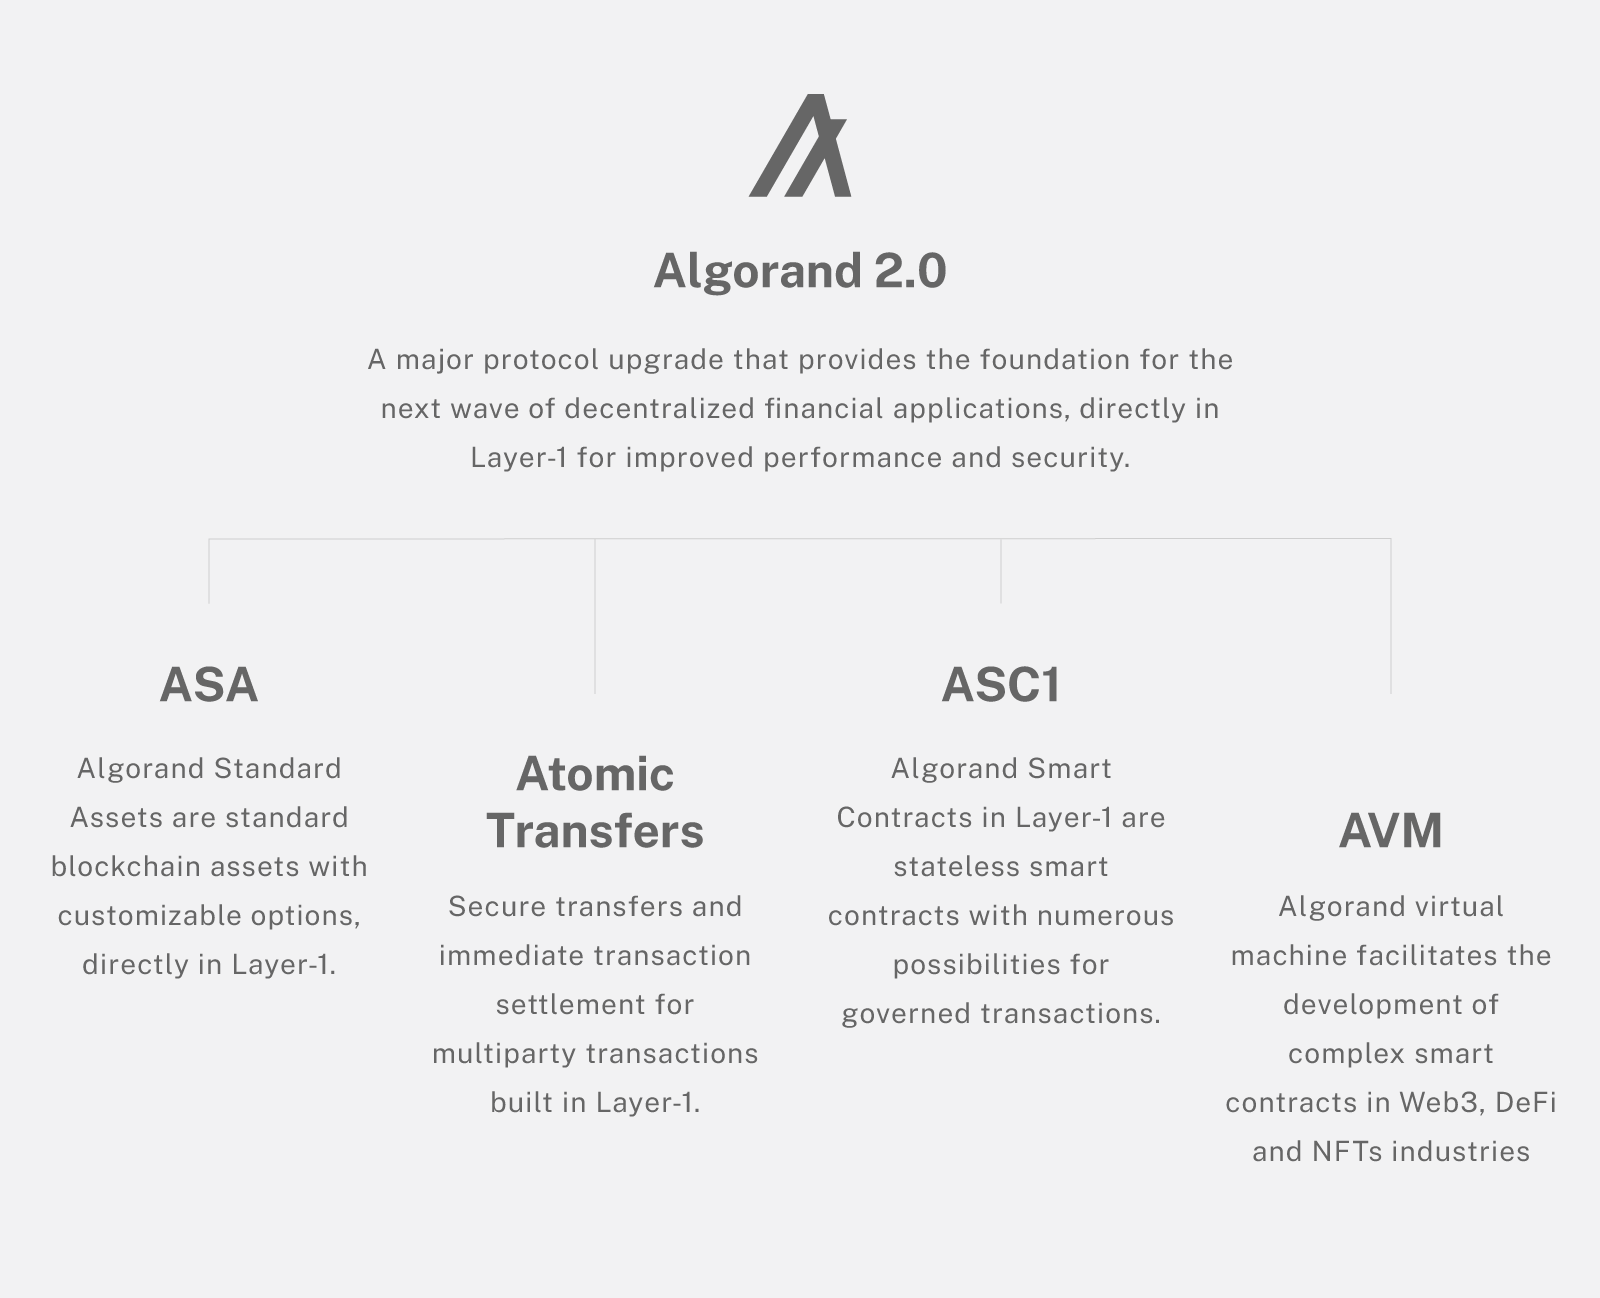
\includegraphics[scale=0.2]{figures/Algorand_primer_content_10 (1).png}  % largura percentual
	\caption{Algorand (ALGO) Research Primer, source: \href{https://21shares.com/research/algorand-research-primer}{21Shares}}
	\label{fig:algoprimer}
\end{figure}

\begin{tcolorbox}[colback=white!20!white,colframe=red!80!black,rounded corners]
\danger An important feature to mention is that Yarilabs created their own Algorand SDK\footnotemark, written in Elixir: the \textit{Algodex}.\newline

Algodex is specifically designed to interact with the Algorand blockchain. It provides developers with a framework and a collection of functions and resources to facilitate the integration of Algorand's features and capabilities into their Elixir-based applications.\newline

By using Algodex, developers can leverage the functionalities of the Algorand blockchain, such as creating and managing accounts, sending and receiving transactions, querying blockchain data, interacting with smart contracts and more. The SDK abstracts away some of the complexities of interacting with the Algorand blockchain, making it easier and more efficient for developers to build Algorand-powered applications using the Elixir programming language.\danger
\end{tcolorbox}

\footnotetext{An SDK (Software Development Kit) is a set of tools, libraries, and documentation that simplifies the development of applications for a specific platform or technology.}

The consensus mechanisms mentioned on section \ref{cons.mec} are incredibly powerful, but Algorand Blockchain takes advantage of another mechanism: Pure Proof-of-Stake (PPoS).

As seen on \href{https://algorand.com/technology/algorand-protocol}{Algorand's technology page}, its consensus mechanism is permissionless (see \ref{typesofb}) and PURE PROOF OF STAKE™.\newline

Algorand's PPoS protocol incorporates Byzantine consensus\footnote{The corresponding Byzantine Consensus is not exactly the same as seen on section \ref{cons.mec}, since there's some variations of the algorithm. For a further understanding, please read paper \cite{algo}}, where the influence of each user on the selection of a new block is directly proportional to their stake (number of tokens) in the system. Random and secret selection of users to propose blocks and vote on block proposals ensures fairness and security. Unlike other approaches, where a small subset of the economy determines the security of the whole economy, Algorand's PPoS ties the security of the entire system to the honesty of the majority. This approach ensures that malicious users holding a small fraction of the money cannot harm the entire network, making Algorand more resilient \cite{alg}.\newline

\textbf{How does PPoS work?} \cite{alg, algo, ppow}\newline

In Algorand, participation is open to all token holders, which \textit{is what makes it a pure proof-of-stake (PPoS) protocol}. Each participant holds a certain number of Algorand tokens (ALGOs) in their wallet, allowing them to engage in the consensus protocol and contribute to the network's security and operations.\newline

\textbf{Protocol Participation:}
To participate in the protocol, users generate and register a participation key, separate from their spending keys, ensuring the security of their tokens even if their participating node is compromised. With the participation key, users can propose and vote on blocks, actively contributing to the consensus process\footnote{This defines the Gossip protocol shown in figures \ref{fig:algo} and \ref{fig:algoflow}.}.\newline

\textbf{Block Proposal:}
During each round of the consensus protocol, a subset of participants is randomly selected to propose a new block. The selection process is based on the number of tokens held by each participant, giving those with a larger stake a higher probability of being chosen as block proposers. This fair and secure selection mechanism ensures that the consensus protocol is inclusive and that participants with a significant stake have a greater influence on block proposal.\newline

\textbf{Block Validation:}
After a block is proposed, a different subset of participants is randomly chosen to validate the block. Validators carefully examine the proposed block for correctness and legitimacy. The selection of validators is determined using a verifiable random function (VRF), ensuring a decentralized and unbiased validation process. Validators play a crucial role in maintaining the integrity of the blockchain by verifying proposed blocks.\newline

\textbf{Soft Vote:}
In the soft vote phase, nodes run the VRF for each participating account they manage to determine if they have been chosen to be part of the soft vote committee. If selected, these accounts contribute weighted votes based on the number of ALGOs they hold. The soft vote committee filters the block proposals down to one by voting to confirm the block with the lowest VRF output calculated at the timeout. These votes, along with the VRF proof, are shared with other nodes, and each node validates the committee membership VRF proof before adding it to the vote tally. Once a quorum is reached for the soft vote, the process advances to the certify vote step.\newline

\textbf{Certify Vote:}
Following the soft vote, a new committee is formed to check the block proposal that received the soft vote for potential issues such as overspending or double-spending. If the block is deemed valid, the committee proceeds to vote on certifying the block. Similar to the soft vote, each node selects a committee from its managed accounts and sends their votes. These votes are collected and validated by each node until a quorum is reached, indicating consensus. Once the block is certified, it is considered final and added to the blockchain.\newline

\textbf{Block Confirmation:}
After the block is certified by a sufficient number of participants, it is confirmed and added to the blockchain. The confirmation process enhances the finality of the block, making it highly unlikely to be reverted. This immutability strengthens the integrity and reliability of the Algorand blockchain.\newline

\textbf{Consensus Agreement:}
Algorand achieves consensus agreement through a decentralized Byzantine Agreement (BA) protocol called Binary Byzantine Agreement (BBA). This protocol enables participants to collectively agree on the block proposal and validation outcome, even in the presence of malicious actors or network issues. By leveraging BBA, Algorand ensures a robust and secure consensus mechanism.\newline

\textbf{Fast and Scalable Block Production:}
Algorand's consensus mechanism enables fast block production, with a new block added to the blockchain approximately every 4.5 seconds. This high throughput rate ensures scalability, enabling the Algorand network to handle a large number of transactions efficiently. The combination of random selection through VRF, the weighted voting system based on stake, and the use of BBA protocol contribute to the fast and secure block production process.\newline

By incorporating the principles of pure proof-of-stake, random selection for block proposal and validation, soft and certify votes, and Byzantine Agreement protocols, Algorand establishes a robust and decentralized consensus mechanism. This approach allows Algorand to provide a high-performance blockchain platform that is secure, scalable and inclusive for all token holders.\newline

Figures \ref{fig:algo} and \ref{fig:algoflow} can be used as an example of what was just explained:\newline

\begin{figure}[htbp]
	\centering
	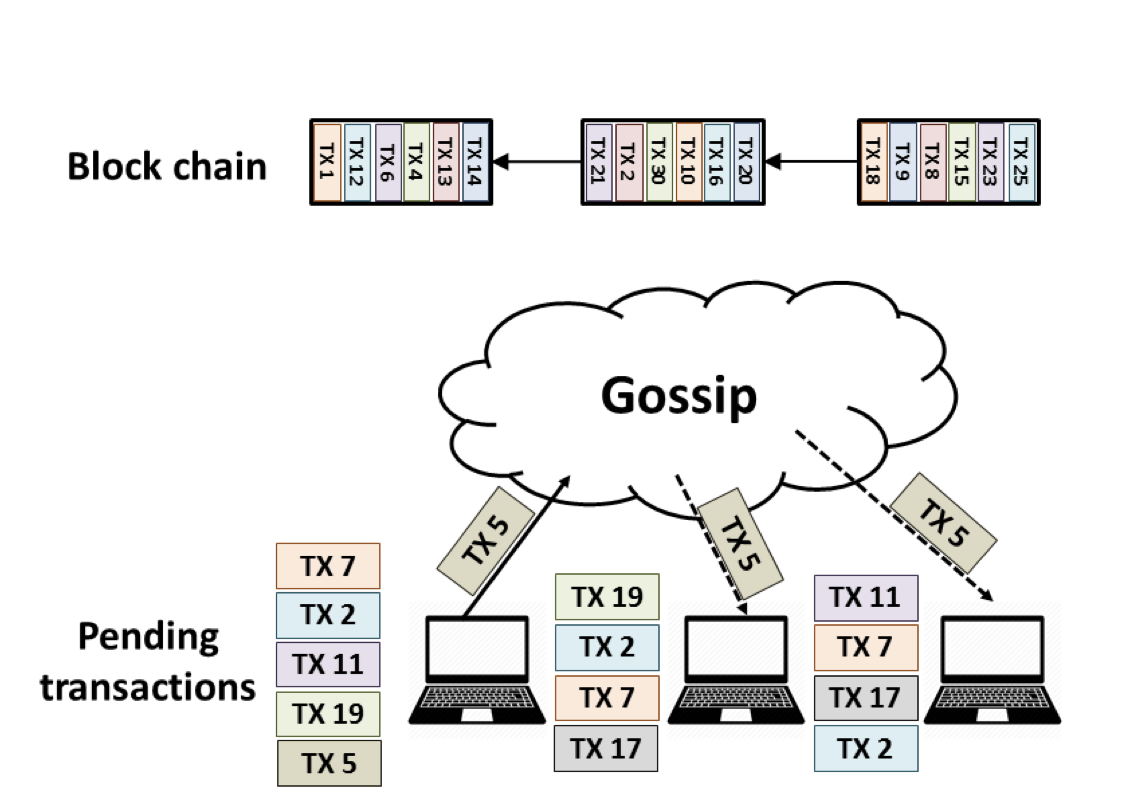
\includegraphics[scale=0.4]{figures/algorand_workflow.png}  % largura percentual
	\caption{Transaction Flow in Algorand, source: \href{https://people.csail.mit.edu/nickolai/papers/gilad-algorand-eprint.pdf}{MIT}}
	\label{fig:algo}
\end{figure}

\begin{figure}[htbp]
	\centering
	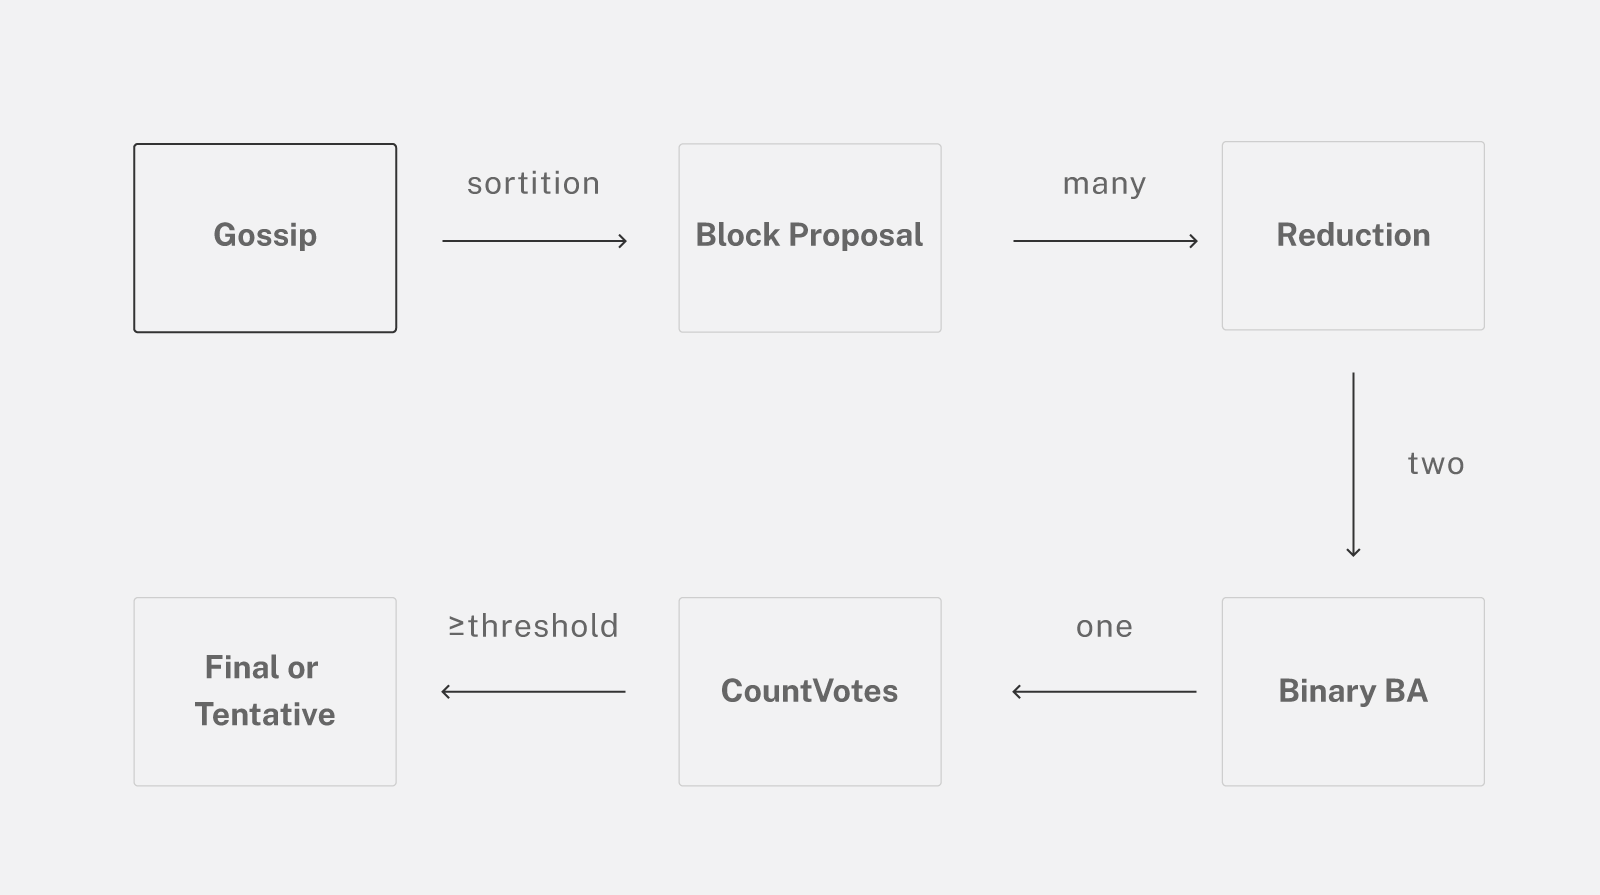
\includegraphics[scale=0.2]{figures/Algorand_primer_content_04.png}  % largura percentual
	\caption{Transaction Flow in Algorand, source: \href{https://21shares.com/research/algorand-research-primer}{21Shares}}
	\label{fig:algoflow}
\end{figure}

\textbf{Advantages over Proof-of-Work (PoW):}\newline

PoW, the consensus mechanism used by Bitcoin and Ethereum, suffers from several limitations. It is highly resource-intensive, requiring specialized hardware and significant energy consumption. In contrast, Algorand's PPoS eliminates the need for resource-intensive mining, making participation accessible to all users without specialized equipment or excessive energy consumption. This reduces barriers to participation and fosters a more inclusive and sustainable network.\newline

Furthermore, PoW systems often lead to a concentration of power in mining pools, risking centralization and potential manipulation. Algorand's PPoS ensures that malicious users gain no advantage by splitting their stake or pooling resources, as influence is solely based on stake proportion. This enhances decentralization and security within the network, eliminating the vulnerability associated with concentrated power.\newline


\textbf{Scalability and Finality:}\newline
Scalability is a critical factor for blockchain protocols aiming to serve a global economy. PoW systems face challenges with block propagation, resulting in slower transaction processing times. In contrast, Algorand's PPoS protocol boasts low computation and communication overhead, enabling rapid block propagation within seconds. This scalability allows Algorand to sustain a high transaction rate, making it suitable for large-scale adoption and real-world financial applications.\newline

Additionally, Algorand's PPoS eliminates the occurrence of forks, ensuring transaction finality. In PoW systems, forks can cause uncertainty and delays, requiring multiple block confirmations to ensure a transaction is valid. Algorand's single block certification mechanism ensures that once a block is added to the chain, transactions within it are considered final, providing immediate transaction certainty and enhancing user confidence.\newline

\subsection{DHARM- Dharma Network's token}

DHARM is the main token of Dharma Network's DApp. It's a stable and mineable token, mined with Proof-of-Real-Work, which is executed by an user on a specific project. It has 8 decimals just like Bitcoin and it's smallest unit is called \textit{nanoDharm} \cite{dharma}.

\begin{equation}
    1 nanoDharm = 0.0000 0001 Dharm
\end{equation}

\textit{Proof-of-Real-Work} shares similarities with the Proof-of-Work (PoW) mechanism used in blockchain networks like Bitcoin. However, there is one major difference: the computational effort expended in DHARM's mining process is directly linked to real-world activities or transactions, distinguishing it from the abstract computational puzzles typically associated with PoW.\newline

Some relevant \textit{blockchain components of Dharma Network} are the following:

\begin{itemize}
    \item \textit{Minter} - TEAL stateless escrow contract that will own the unminted tokens (will be the new DHARM reserve account)
    \item \textit{Dharma Scriber} - TEAL stateful smart contract that miners need to opt-in. Scriber writes to users local-state how much Dharm they mined, bonus mining rewards and verification data. It’s also responsible to reset the local-state when users claim their DHARM successfully on an atomic swap with the minter
    \item \textit{Dharma Oracles} - writes DHARM blocks information into the Algorand Blockchain. The exchange rates for DHARM/ALGO are also published by the oracle
    \item \textit{Organization Escrows} - Every organization has its own smart contract to hold the funds of the funding rounds
    \item \textit{Rewards Calculator} - responsible to calculate mining rewards. Calls the Dharma Scriber to write rewards to users local-state
    \item \textit{Treasury Account (dharma.algo)} - receives the funds from the organization escrows contracts when a funding round is closed successfully \cite{dharma}.
\end{itemize}

\textbf{DHARM's mining process}\newline

DHARM's mining process is implemented in a secured and decentralized manner called ASA (Algorand Standard Asset).\newline

ASA is an on-chain asset that benefit from the same level of security and ease of use as Algo\footnote{Algo is Algorand's native utility token.}. With the help of these, such things as stablecoins, loyalty points and system credits can be represented. Single assets, such as a deed for a house or collectable items, can also be represented. ASAs have a wide range of use cases, allowing for the representation of both fungible and non-fungible assets with varying degrees of control. \newline

ASAs offer several important concepts that developers need to understand when working with them. Some of those concepts are:

\begin{enumerate}
    \item \textbf{ASA Transaction Types and User Flows:}

    There are three primary transaction types associated with ASAs: \textit{AssetConfigTxn (acfg)}, \textit{AssetFreezeTxn (afrz)}, and \textit{AssetTransferTxn (axfer)}. Each transaction type serves a specific purpose and, combined with different parameter specifications, supports seven primary user flows:

    \begin{itemize}
        \item \textit{Asset Creation:} Creating a new asset on the Algorand blockchain.
        \item \textit{Asset (Re-)Configuration:} Modifying the configuration of an existing asset, such as changing its name or total supply.
        \item \textit{Asset Freezing:} Enabling the freezing of assets, allowing certain accounts to control the ability to trade the asset.
        \item \textit{Asset Destruction:} Removing an existing asset from the blockchain.
        \item \textit{Asset Transfer:} Transferring assets between accounts.
        \item \textit{Asset Revocation:} Revoking assets from a specific account and transferring them to another account.
        \item \textit{Asset Opt-In:} Allowing an account to receive a new type of asset.
    \end{itemize}

    Each one of these transaction types and user flows is more detailed in figure \ref{fig:asa}:

    \begin{figure}[htbp]
	   \centering
	   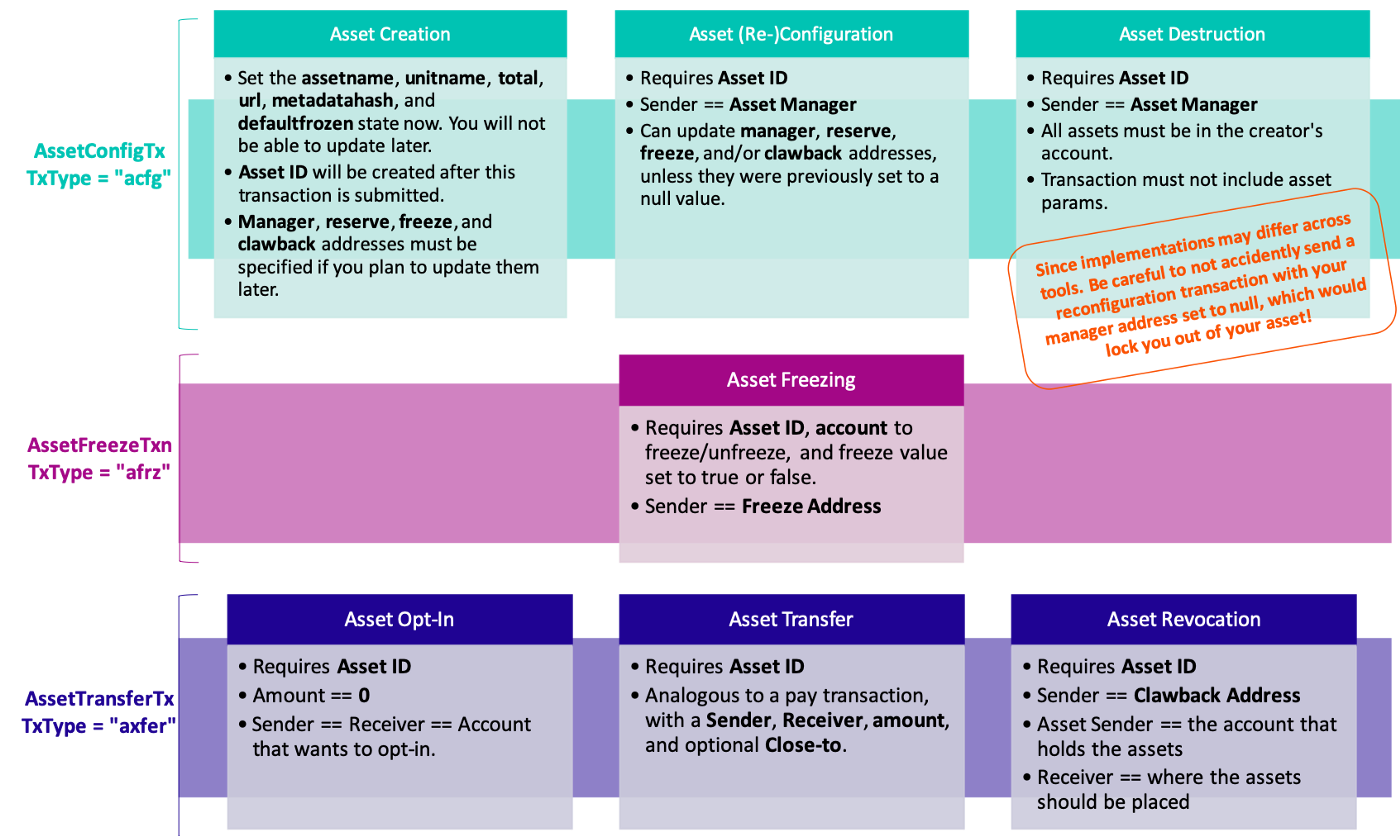
\includegraphics[scale=0.2]{asa}  % largura percentual
	   \caption{ASA Transaction Types, source: \href{https://developer.algorand.org/articles/algorand-standard-assets/}{Algorand's Developer Portal}}
	   \label{fig:asa}
    \end{figure}

    
    \item \textbf{Asset Opt-Ins:}

    To receive a new type of asset, an account must opt-in. This process involves sending a 0-amount transfer of the desired asset from and to the account itself. By opting-in, a holding for the new asset is created in the account, enabling others who own that asset to transfer it to the account.

    \item \textbf{Minimum Balance Requirement:}

    Every Algorand address on the ledger must maintain a minimum balance of 100,000 microAlgos. When an account opts-in to receive an ASA, the minimum balance increases by 100,000 microAlgos. For example, if an account opts-in to receive two different ASAs, the minimum balance will be 300,000 microAlgos (100,000 microAlgos x 2 ASAs + 100,000 microAlgos for the native Algo).


    \item \textbf{Freeze Assets:}

    Upon asset creation, it is possible to specify a freeze address and a defaultfrozen state. Setting the defaultfrozen state to true requires the corresponding freeze address to issue unfreeze transactions, allowing trading of the asset to and from specific accounts. This feature can be useful for implementing checks like KYC/AML requirements. Conversely, setting the defaultfrozen state to false allows anyone to trade the asset, and freeze transactions can be issued by the freeze address to disallow trading for specific accounts. To ensure asset holders that the asset will never be frozen, the defaultfrozen state can be set to false, and the freeze address can be set to null or an empty string.

    \item \textbf{Revoke Assets:}

    ASAs also offer the ability to revoke assets from specific accounts using a clawback address. If specified, the clawback address can revoke the asset from any account and transfer it to another account that has previously opted-in. This feature is valuable in situations where asset holders breach certain terms or conditions established for the asset. Similar to freezing, the clawback address can be set to null if it is desirable to ensure that asset revocation is not possible.

    
\end{enumerate}



ASAs are supported at the protocol level on the Algorand Blockchain. When an ASA is created, the entire supply is automatically generated and becomes immediately available. However, ASAs do not natively support incremental mining.\newline

To address this, the Dharma Network has implemented a stateless escrow contract called the Minter. The Minter acts as the sole entity responsible for transferring Dharm tokens to miners. Instead of having a reserve account controlled by a central entity, the Minter holds the unminted tokens and ensures their secure distribution.

To request Dharm tokens from the Minter, an account that has opted into Dharm must create a transaction as part of a grouped atomic transaction. This transaction must include:

\begin{enumerate}
    \item A request to the Minter for Dharm tokens, accompanied by proof in the local state that the user is entitled to receive those tokens.
    \item A call to the Dharma Scriber smart contract to reset the state.
\end{enumerate}

Algorand supports atomic transactions (see figure \ref{fig:algoprimer}), meaning that if any of the transactions within a grouped atomic transaction fails, all of them fail. Therefore, the Minter checks that the miners have used a group transaction, are eligible to receive Dharm tokens, and that the Scriber contract was successfully called. This ensures the integrity and correctness of the mining process.\newline

The use of atomic transactions, in combination with the Proof of Real Work mechanism described in the additional information, adds an extra layer of security to the mining process. The activity transactions related to mining are stored on an immutable chain of blocks, making the entire mining process secure and publicly verifiable.\newline


\textbf{Dharma Network's DAO:}\newline

The Dharma Network embraces a decentralized approach to governance and recognizes the importance of establishing a strong foundation to support its operations. To this end, the Dharma Network Foundation will be set up to provide legal support in the formation of a \textit{Decentralized Autonomous Organization} (DAO) for DHARM \cite{dharma}.\newline

A DAO, or Decentralized Autonomous Organization, is a concept that leverages blockchain technology to create an organization that operates in a decentralized and autonomous manner. It is designed to eliminate the need for traditional centralized management structures and instead relies on smart contracts and distributed consensus mechanisms to govern and execute its operations.\newline

The purpose of a DAO is to enable a group of individuals or participants to collectively make decisions, manage resources and execute actions without relying on a central authority. By leveraging blockchain's transparency, immutability and decentralized nature, a DAO aims to create a trustless and efficient system that operates based on predefined rules and algorithms.\newline

The key features and purposes of a DAO include \cite{dao, dao2, dao3}:

\begin{itemize}
    \item \textit{Decentralization:} A DAO operates on a decentralized network, typically a blockchain, where no single entity or individual has control over the organization's operations or decision-making. Instead, decision-making power is distributed among participants based on predetermined rules.
    \item \textit{Autonomy:} A DAO is designed to be autonomous, meaning it can perform predefined actions and execute transactions without requiring direct human intervention. Smart contracts, which are self-executing agreements with the terms of the agreement directly written into code, enable this autonomy.
    \item \textit{Governance:} DAOs allow participants to collectively make decisions through voting mechanisms. Each participant typically has voting power proportional to their stake or ownership in the organization, allowing for democratic decision-making processes.
    \item \textit{Resource Management:} DAOs can manage and allocate resources based on predefined rules and algorithms encoded in smart contracts. This can include managing and distributing funds, assets, or tokens held by the organization.
    \item \textit{Transparency:} As DAOs are built on blockchain technology, all transactions, decisions, and changes to the organization's state are recorded on the public ledger. This transparency ensures that all participants can audit and verify the actions and transactions within the organization.
    \item \textit{Trustlessness:} DAOs aim to eliminate the need for trust between participants by relying on the transparency and immutability of blockchain technology. All actions and operations are recorded on the blockchain, and smart contracts execute based on predefined rules, removing the need for trust in individual participants.
\end{itemize}

The overall difference of DAO and traditional organizations is represented on figure \ref{fig:dao}:

    \begin{figure}[htbp]
	   \centering
	   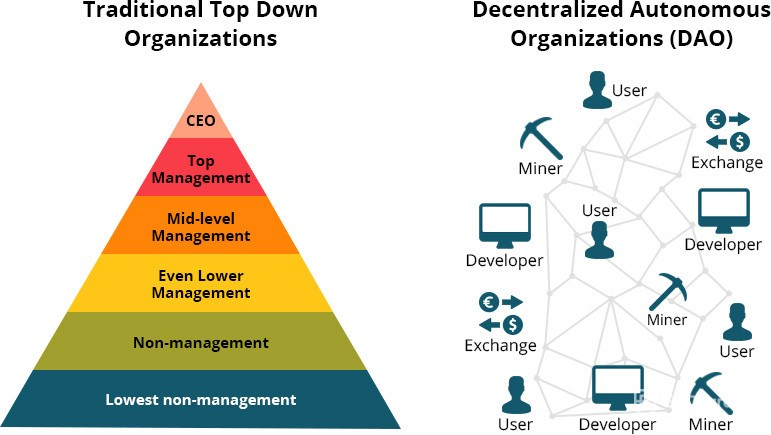
\includegraphics[scale=0.4]{figures/dao.png}  % largura percentual
	   \caption{Difference between Traditional Organizations and Decentralized Autonomous Organizations, source: \href{https://academy.moralis.io/blockchain-guides/beginners-guide-how-to-create-a-dao}{Moralis Academy}}
	   \label{fig:dao}
    \end{figure}

The Dharma Network DAO will be the governing body of the ecosystem, allowing all Dharm token holders to participate in the decision-making process through voting on DAO proposals. This model draws inspiration from the successful implementation of Algorand Governance. By granting token holders voting rights, the DAO ensures that decisions are made in a democratic and inclusive manner, reflecting the collective will of the community.\newline

The responsibilities of the Dharma DAO will encompass various aspects of the network's operations. These include determining which liquidity pools to create, managing liquidity by adding or removing assets, adjusting bonus mining rewards, setting limits for mining activities, and distributing fees. The DAO will play a crucial role in shaping the ecosystem by making informed decisions on these matters.\newline

As the project progresses and achieves a phase of high liquidity, the Dharma DAO will have the ability to open grants for projects that align with the goals and values of the DAO and the Dharma Network as a whole. These projects would need to meet specific criteria, such as having automated activity tracking and bringing value to the ecosystem and the world at large. By providing funding opportunities to promising projects, the DAO aims to foster innovation and collaboration within the Dharma Network.\newline

The funding rounds initiated by the Dharma DAO (DAO funding round) will introduce a unique approach to collateralization. Unlike other funding rounds that require full collateralization, DAO funding rounds may adopt a partial collateralization scheme, such as 25\%/ 75\%, 50\%/ 50\% or 0\%/ 100\%. In these rounds, projects seeking funding will contribute a portion of the collateral and the remaining portion will be granted in mining rewards based on automated activity tracking. This innovative funding mechanism aims to incentivize project participation and align the interests of the project with the overall success of the Dharma Network \cite{dharma}.\newline

It is important to note that the concept of the Dharma DAO and its funding mechanisms will be further developed and detailed in the future. As the Dharma Network evolves and matures, the DAO will continue to play a crucial role in shaping the direction of the ecosystem, promoting collaboration and supporting projects that contribute to the growth and development of the Dharma Network.\newline

\section{Existing Solutions}

While the DeFi landscape is constantly evolving, Dharma Network stands out as a unique solution that combines the power of the Algorand blockchain with innovative mining mechanisms. Existing solutions often rely on centralized systems or lack the level of transparency and decentralization offered by Dharma Network.\newline

However, let's take a look to projects that might have some similarities with Dharma Network.\newline

There are many DAOs based on Algorand, such as \href{https://algorand.com/pt/ecosystem/use-cases/staker-dao}{StakerDAO}, \href{https://algodao.fi}{AlgoDAO} and \href{https://www.algorand.foundation/news/kinn-grant-award}{Kinn DAO}. 

\subsection{Pi Network}

\href{https://minepi.com}{\textit{Pi Network}} is a mobile app-based project that allows users to mine a native cryptocurrency called \textit{Pi} by simply interacting with the app on a daily basis. Similar to Dharma Network, \textit{Pi Network} aims to create a decentralized network of users and incentivize their participation through mining activities. 

\subsection{Steemit}

\href{https://steemit.com}{\textit{Steemit}} is a blockchain-based social media platform that allows users to create and share content while earning rewards in the form of the platform's native cryptocurrency called \textit{STEEM}. Users can contribute by creating blog posts, articles, and other forms of content, and their contributions are rewarded based on the engagement and popularity of their content.\newline

The platform uses a consensus algorithm called \textit{Delegated Proof of Stake} (DPoS), where users can "mine" or earn \textit{STEEM} tokens by staking their existing tokens and participating in the block validation process. Users with more stake have a higher probability of being chosen as block validators and earning rewards.\newline

In addition to earning rewards through content creation and mining, Steemit also has a voting system where users can upvote or downvote content they find valuable or not. These votes not only determine the visibility and popularity of the content but also contribute to the rewards received by the content creators.\newline

Steemit offers a unique way for users to earn cryptocurrency by participating in the platform's activities and engaging with the community. It combines social media features with blockchain technology, creating an incentivized ecosystem where users are rewarded for their contributions \cite{steemit}.\newline

\subsection{Brave Browser}

\textit{Brave Browser} is a privacy-focused web browser that incorporates blockchain technology and a token economy to reward users for their attention and engagement with online advertisements. The browser blocks unwanted ads and trackers by default, providing a faster and more secure browsing experience.\newline

Brave Browser introduces the \href{https://brave.com/brave-rewards/}{\textit{Basic Attention Token}} (BAT) as its native cryptocurrency. Users have the option to opt-in to view privacy-respecting ads while using the browser. When users choose to view these ads, they are rewarded with BAT tokens. The rewards are distributed based on user attention and engagement with the ads, ensuring a fair compensation model.\newline

Additionally, \textit{Brave Browser} allows users to support their favorite content creators directly through BAT token contributions. Users can allocate a portion of their earned BAT tokens to the websites and content creators they appreciate, providing an alternative monetization model for online content.\newline

By integrating blockchain technology and a token-based economy, \textit{Brave Browser} creates a decentralized ecosystem where users are incentivized to engage with advertisements and support content creators, all while maintaining their privacy and control over their data.\newline

\subsection{Gitcoin}

\href{https://www.gitcoin.co}{\textit{Gitcoin}} is a platform that connects developers with open-source projects and provides a way for them to earn rewards for their contributions. It is built on the Ethereum blockchain and utilizes smart contracts to facilitate transparent and incentivized collaboration within the open-source community.\newline

Key features of \textit{Gitcoin} include \cite{gitcoin}:

\begin{itemize}
    \item \textit{Funding Open-Source Projects:} Gitcoin enables individuals and organizations to financially support open-source projects they find valuable. Through the platform, users can contribute funds to specific projects or initiatives they wish to support.
    \item \textit{Bounties:} Gitcoin allows project maintainers to create bounties for specific tasks or issues within their projects. Developers can then choose to work on these bounties and receive rewards upon successful completion. This incentivizes developers to contribute their skills and expertise to the projects that interest them.
    \item \textit{Hackathons and Grants:} Gitcoin hosts online hackathons and facilitates grants to support the development of new projects and ideas. These events encourage collaboration, innovation, and the creation of impactful solutions within the open-source ecosystem.
    \item \textit{Reputation and Recognition:} Gitcoin incorporates a reputation system that tracks and showcases the contributions made by developers. This reputation can help developers establish credibility within the community and increase their chances of receiving more significant bounties or grants.
    \item \textit{Gas Optimization:} Gitcoin uses a mechanism called "gas optimization" to reduce transaction costs and improve efficiency when interacting with the Ethereum blockchain. This optimization helps to minimize the overhead associated with executing transactions on the network.
\end{itemize}

\textit{Gitcoin} aims to foster a sustainable open-source ecosystem by providing a platform where developers can get paid for their work and where open-source projects can receive financial support. It creates opportunities for collaboration, innovation, and community-driven development.\newline

The platform has gained popularity within the blockchain and Ethereum communities, but it also supports projects beyond the blockchain space. As for the previously seen projects, \textit{Gitcoin} is the most similar one to Dharma Network for now.



	

